% \documentclass{article}
% \usepackage{beamerarticle}
\documentclass{beamer}
% Beamer theme settings
\usetheme{Madrid}
\usecolortheme{default}
\usepackage{amsmath}
\usepackage{tikz}
\usepackage{mathtools}
\usepackage{hyperref}
\usetikzlibrary{intersections}
\usepackage{graphicx}
\usepackage{svg}
\usepackage{xcolor}



% Define commands for vectors
\newcommand{\va}{\mathbf{a}}
\newcommand{\vb}{\mathbf{b}}
\newcommand{\vc}{\mathbf{c}}
\newcommand{\vd}{\mathbf{d}}
\newcommand{\ve}{\mathbf{e}}
\newcommand{\vv}{\mathbf{v}}
\newcommand{\vu}{\mathbf{u}}
\newcommand{\vw}{\mathbf{w}}
\newcommand{\vx}{\mathbf{x}}
\newcommand{\vy}{\mathbf{y}}
\newcommand{\vz}{\mathbf{z}}
\newcommand{\N}{\mathbb{N}}
\newcommand{\Z}{\mathbb{Z}}
\newcommand{\R}{\mathbb{R}}
\newcommand{\Q}{\mathbb{Q}}
\newcommand{\rank}{\text{rank}}







% Title page

\title[Lecture 7]{Gradient, Hessian}
\author[Aprikyan, Tarkhanyan]{Hayk Aprikyan, Hayk Tarkhanyan}
\institute[ACA]{Armenian Code Academy}
\date{November 18, 2024}

\begin{document}

\begin{frame}
  \titlepage
\end{frame}





% slide 5: gradient
\begin{frame}{Gradient}
So far, we have been considering functions of one variables. Now let's suppose $f(x,y)$ or, more generally, $f(x_1,x_2,\dots,x_n)$ depends on $n$ variables.
\pause
  \begin{block}{Definition}
        The following limit:
        \[
        \frac{\partial f}{\partial x} = \lim_{{h \to 0}} \frac{f(x + h, y) - f(x, y)}{h}
        \]
        if exists and finite, is called the \textbf{partial derivative} of the function \(f(x, y)\) with respect to \(x\), and is denoted by $\frac{\partial f}{\partial x}$ or $f_x$.
        
        Similarly, the partial derivative with respect to \(y\) is denoted by \(\frac{\partial f}{\partial y}\) or $f_y$, and defined as:
        \[
        \frac{\partial f}{\partial y} = \lim_{{h \to 0}} \frac{f(x,y + h) - f(x, y)}{h}
        \]
    \end{block}


\end{frame}


% slide 5: gradient
\begin{frame}{Gradient}

    \begin{exampleblock}{Example}
        If \(f(x, y) = x^2 + y^2\), then:
        \[
        \frac{\partial f}{\partial x} = 2x \quad \text{and} \quad \frac{\partial f}{\partial y} = 2y
        \]
    \end{exampleblock}
\pause 
        The partial derivative is the rate of the function change with respect to one of the variables, treating the other variables as constants.
\pause
 \begin{block}{Definition}
        The row vector, the components of which are the partial derivatives of $f(x,y)$, is called the \textbf{gradient} of the function \(f(x, y)\), and denoted by \(\nabla f\) or $\text{grad} f$:
        \[
        \nabla f = \left[\frac{\partial f}{\partial x}\quad  \frac{\partial f}{\partial y}\right]
        \]
    \end{block}
In the example above, $        \nabla f = [2x\quad 2y]$.

\end{frame}



% slide 5: gradient
\begin{frame}{Gradient}
Similarly, for a function of $n$ variables, $f(x_1,\dots,x_n)=f(\vx)$ we define the partial derivatives as:
\[
f_{x_1}(\vx) = \frac{\partial f}{\partial x_1}(\vx) = \lim_{{h \to 0}} \frac{f(x_1 + h, x_2, \ldots, x_n) - f(x_1, x_2, \ldots, x_n)}{h},
\]
\[
f_{x_2}(\vx) = \frac{\partial f}{\partial x_2}(\vx) = \lim_{{h \to 0}} \frac{f(x_1, x_2+h, \ldots, x_n) - f(x_1, x_2, \ldots, x_n)}{h},
\]
\[
\vdots
\]
\[
f_{x_n}(\vx) = \frac{\partial f}{\partial x_n}(\vx) = \lim_{{h \to 0}} \frac{f(x_1, x_2, \ldots, x_n + h) - f(x_1, x_2, \ldots, x_n)}{h}.
\]

And the gradient of $f(\vx)$ as:
\[
\nabla f = \frac{df}{d\vx} =
\begin{bmatrix}
\frac{\partial f(\vx)}{\partial x_1} & \frac{\partial f(\vx)}{\partial x_2} & \ldots & \frac{\partial f(\vx)}{\partial x_n}
\end{bmatrix}
\in \mathbb{R}^{1 \times n}
\]

\end{frame}



% slide 5: gradient
\begin{frame}{Gradient}
% Similar to derivatives of one-variable functions, partial derivatives have the following
\begin{block}{Properties}
    \begin{enumerate}
        \item \[\frac{\partial}{\partial x_i} (f(\vx) \pm g(\vx)) = \frac{\partial f(\vx)}{\partial x_i} \pm \frac{\partial g(\vx)}{\partial x_i}\]
        
        \item \[\frac{\partial}{\partial x_i} (c \cdot f(\vx)) = c\cdot\frac{\partial f(\vx)}{\partial x_i} \]

        \item \[\frac{\partial}{\partial x_i} (f(\vx) \cdot g(\vx)) = \frac{\partial f(\vx)}{\partial x_i} \cdot g(\vx) + f(\vx) \cdot \frac{\partial g(\vx)}{\partial x_i}
\]
    \end{enumerate}
\end{block}
\pause
\begin{example}
    Let \( f(x,y)=f(\vx) = \color{blue}{2x^2} \) and \( g(x,y)=g(\vx) =\color{purple}{4x + 6y} \).

\begin{center}
    $(f\cdot g)_{x} = \color{blue}{2x^{2}}\color{purple}{(4)} \color{black}{+} \color{purple}{(4x + 6y)}\color{blue}{(4x}) \color{black}{= 24x^{2} + 24xy}$\\
    $(f\cdot g)_{y} = \color{blue}{2x^{2}}\color{purple}{(6)} \color{black}{+} \color{purple}{(4x + 6y)}\color{blue}{(0}) \color{black}{= 12x^{2}}$
\end{center}

\end{example}

\end{frame}

% slide 6: chain rule
\begin{frame}{Chain Rule}
Let $z$ be a function of $x$ and $x$ be a function of $t$. Then
$$\frac{dz}{dt} =\frac{dz}{dx}\cdot \frac{dx}{dt}
$$

\pause This rule is called the \textbf{chain rule}.

\pause
\begin{example}
    Let $z(x) = x^2 + 4x$ where $x(t) = 5t^3 + 2t$. \pause To calculate $\frac{dz}{dt} $ we can either substitute the value of $x$ in $z$, expressing $z$ in terms of $t$ and then calculating the limit ($z(t)=( 5t^3 + 2t)^2 + 4( 5t^3 + 2t) = \dots$), \pause or we can use the chain rule: 
\[\frac{dz}{dt} = \frac{dz}{dx} \cdot \frac{dx}{dt}= (2x+4)\cdot (15t^2+2)=(2\cdot (5t^3 + 2t)+4)\cdot (15t^2+2)\]\[=150 t^5 + 80 t^3 + 60 t^2 + 8 t + 8
        \]
    
\end{example}

\end{frame}


% slide 7: chain rule
\begin{frame}{Chain Rule}
For functions with multiple variables, the chain rule is pretty much the same:
\pause
          \begin{center}

    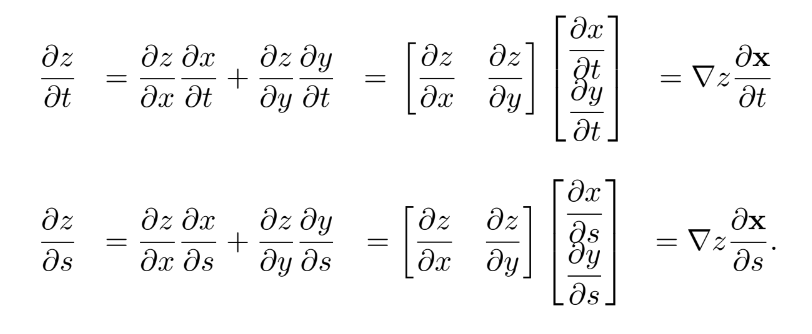
\includegraphics[width=0.9\textwidth, height=\textheight, keepaspectratio]{chain.png}
  \end{center}
\pause
          \begin{center}

    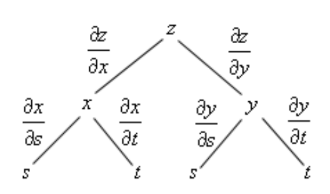
\includegraphics[width=0.3\textwidth, height=\textheight, keepaspectratio]{chain21.png}
  \end{center}
\end{frame}



% slide 7: chain rule
\begin{frame}{Chain Rule}
\begin{example}
    Let $z
=
\sin
(
x^2
+
y^2
)
,
  \:
x
=
t^2
+
3
,\: y
=
t^3$.
\begin{align*}
{dz\over dt}&={\partial z\over \partial x}{dx\over dt}+ {\partial z\over \partial y}{dy\over dt}=(2x \cos(x^2+y^2))\cdot (2t)+(2y \cos(x^2+y^2))\cdot(3t^2)\\&=4xt\cos(x^2+y^2)+6yt^2\cos(x^2+y^2)
\end{align*}
\end{example}
\end{frame}


% slide 8: dir grad
\begin{frame}{Directional Derivative}
When calculating the gradient of a function, we consequently take the rate of change of each coordinate ($x_1, x_2,$ etc), while fixing all other coordinates. What if we change all coordinates simultaneously?\pause

\begin{block}{Definition}
Let $f(\vx)=f(x_1,\dots,x_n)$ be a function, and $\vv=[v_1, \ldots, v_n]$ be any vector with $\|\vv\|=1$. \pause The following limit:
\[\nabla_{\mathbf{v}}{f}(\mathbf{x}) = \lim_{h \to 0}{\frac{f(\mathbf{x} + h\mathbf{v}) - f(\mathbf{x})}{h}}\]
if exists, is called the \textbf{directional derivative} of $f$ along the vector $\vv$.
% \end{block}
\pause
% \begin{block}{Theorem}
    If $f(\vx)$ is differentiable at point $\vx_0$, then
    \[\lim_{{h \to 0}} \frac{f(\vx_0 + h\vv) - f(\vx_0)}{h} = \frac{\partial f}{\partial x_1}(\vx_0) v_1 + \ldots + \frac{\partial f}{\partial x_n}(\vx_0) v_n = \nabla f(\vx_0) \cdot \vv\]
    % (where the last $$ represents the dot product).
\end{block}
\pause - \color{blue} \href{https://www.geogebra.org/m/Bx8nFMNc}{Play with directional derivative!}
\end{frame}


% slide 8: dir grad
\begin{frame}{Directional Derivative}
How is the directional derivative related to gradient? \pause
As we know,
\begin{equation*}
\nabla_{\vv}f=\nabla f\cdot \vv=\|\nabla f\|\cdot \|\vv\| \cdot \cos\theta= \|\nabla f\|\cos\theta
\end{equation*}
where $\theta$ is the angle between $\vv$ and $\nabla f$. \pause
     \vspace{0.3cm}

This expression has its maximum value (i.e. the rate of change of $f$ is the biggest) when $\cos \theta=1$. It happens when the direction of derivative, $\vv$, coincides with the direction of $\nabla f$, the gradient. \pause Therefore,

\begin{block}{Theorem}
    The gradient is the \textit{fastest increasing direction} of the
function.
\end{block}
\pause Similarly, $-\nabla f$ is the fastest decreasing direction of the function.
\end{frame}


% slide 9: extrema 
\begin{frame}{Extrema of a Function}
How can we find the maximum and minimum values of a multivariable function $f(\vx)=f(x_1,\dots,x_n)$?\pause

\begin{block}{Definition}
    $\vx_0$ is called a \textbf{local maximum (minimum)} point of $f$ if there exists a positive number $\delta>0$ such that for all $\vx$ if $\|\vx-\vx_0\|< \delta$, then  $f(\vx) \leq f(\vx_0)$ $\, (f(\vx) \geq f(\vx_0))$.
\end{block}\pause

\begin{block}{Theorem}
    If $\vx_0$ is a local extremum point of $f$ and there exists $\nabla f(\vx_0)$, then $\nabla f(\vx_0) = \textbf{0}$. (The converse is not true).
\end{block}\pause


\begin{block}{Definition}
    $\vx_0$ is called a \textbf{saddle point} of $f$ if $\nabla f(\vx_0) = \textbf{0}$ but it's not an extremum point.
\end{block}

\end{frame}


% slide 9: extrema 
\begin{frame}{Extrema of a Function}
      \begin{center}

    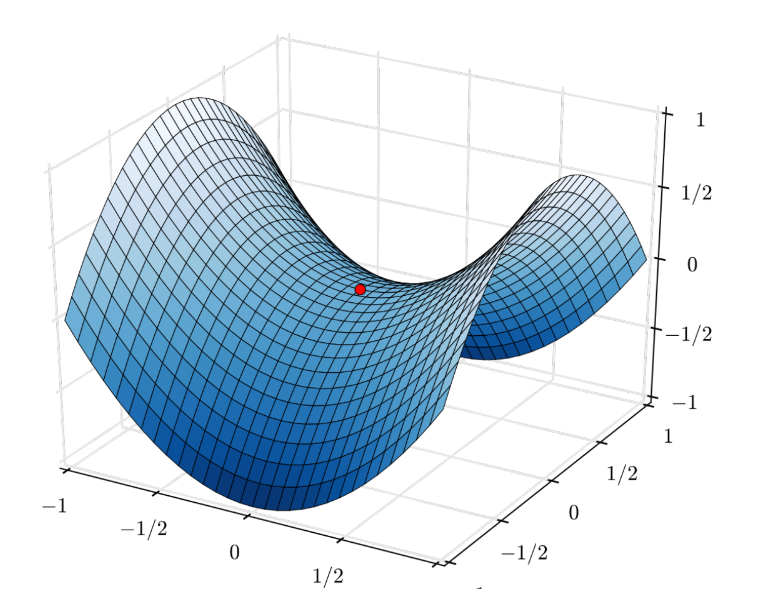
\includegraphics[width=0.8\textwidth, height=\textheight, keepaspectratio]{saddle.png}
  \end{center}
\end{frame}



% slide 9: extrema 
\begin{frame}{Extrema of a Function}
For the functions of one variable we looked at the sign of $f''$. In the case of multivariable functions, we want to look at the "gradient" of $\nabla f$.\pause
\begin{block}{Definition}
    If all second partial derivatives of \( f(\vx) \) exist and are continuous, then the $(n\times n)$ matrix $H$ with entries:
\[
H_{i,j} = \frac{\partial^2 f}{\partial x_i \partial x_j}, \quad i, j = 1, \ldots, n
\]
is called the \textbf{Hessian matrix} of \( f \).
\end{block}
\pause Note that in this case $ \dfrac{\partial^2 f}{\partial x_i \partial x_j}= \dfrac{\partial^2 f}{\partial x_j \partial x_i}$ for any $i,j$.

\end{frame}


% slide 9: extrema 
\begin{frame}{Extrema of a Function}

\begin{example}
    
    Let \( f(x, y) = x^2 + 3xy -y^2 \). 

The second-order partial derivatives of \( f \) are:
\[
\frac{\partial^2 f}{\partial x^2} = 2, \quad
\frac{\partial^2 f}{\partial y^2} = -2, \quad
\frac{\partial^2 f}{\partial x \partial y} = \frac{\partial^2 f}{\partial y \partial x} = 3.
\]

The Hessian matrix is:
\[
H = 
\begin{bmatrix}
2 & 3 \\
3 & -2
\end{bmatrix}
\]

\end{example}
\pause

\begin{block}{Property}
The Hessian matrix is symmetric.
\end{block}\pause
\begin{block}{Theorem}
   If \( f \) is convex, then its Hessian matrix is positive semi-definite.
\end{block}
\end{frame}



% slide 9: extrema 
\begin{frame}{Extrema of a Function}
      \begin{block}{Theorem}
          Let \( f(\vx) \) be any function and \( \vx_0 \) is its critical point. If all second partial derivatives of \( f \) exist and are continuous at \( \vx_0 \), then

\begin{enumerate}
    \item If \( H(\vx_0) \) is positive definite, then \( f \) has a local minimum at \( \vx_0 \).
    \item If \( H(\vx_0) \) is negative definite, then \( f \) has a local maximum at \( \vx_0 \).
    \item If \( H(\vx_0) \) is indefinite (i.e. it has both positive and negative eigenvalues), then \( \vx_0 \) is a saddle point for \( f \).
\end{enumerate}
      \end{block}



\end{frame}

% % slide 4: derivative
% \begin{frame}{Derivative}
%       \begin{center}

%     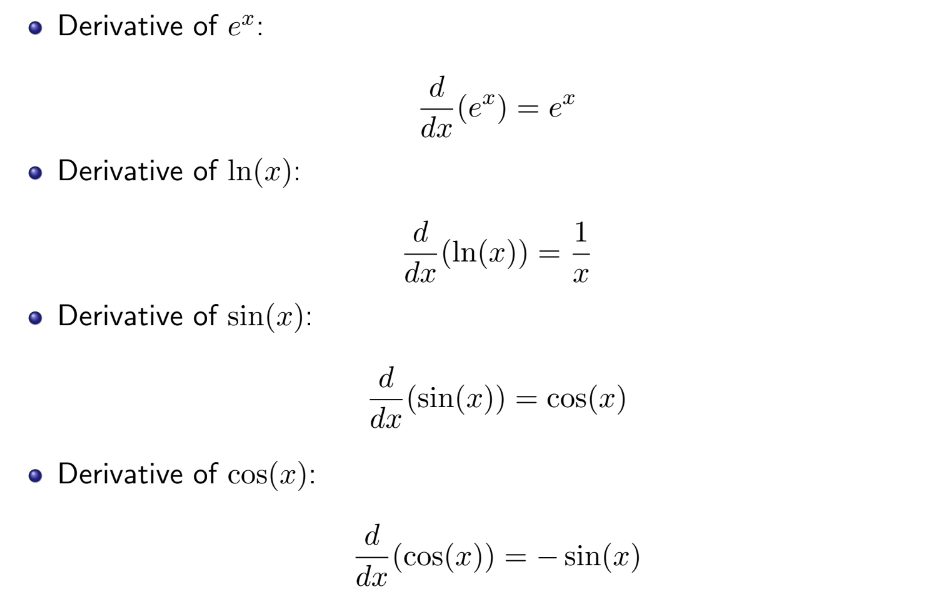
\includegraphics[width=0.9\textwidth, height=\textheight, keepaspectratio]{der2.png}
%   \end{center}
% \end{frame}



% % slide 5: extrema
% \begin{frame}{Extrema of a Function}

% % \begin{center}
% \begin{exampleblock}{Example}
%     Which points are the local extremum points of the following functions? \\ \bigskip
% % \\\includesvg[ width=0.31\textwidth, keepaspectratio]{image-295}\pause 
%  \includesvg[ width=0.31\textwidth, keepaspectratio]{image-296}\pause
%  \includesvg[ width=0.31\textwidth, keepaspectratio]{image-297}\pause
%  \includesvg[ width=0.31\textwidth, keepaspectratio]{image-290}
% \end{exampleblock}
%   % \end{center}
% \pause
% \begin{block}{Theorem}
% If a function \(f\) is continuous on a \textit{closed interval} \([a, b]\), then \(f\) has both a global maximum and a global minimum on \([a, b]\).
    
% \end{block}

  
% \end{frame}


\end{document}
